\setcounter{step}{0}

\subsection{ Kapustnica }

\begin{ingredient}
  
      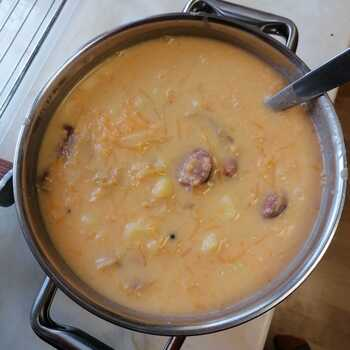
\includegraphics[height=5.5cm]{images/kapustnica}
  
  \def\portions{  }
  \textbf{ {\normalsize Ingrediencie (4 porcie):} }

  \begin{main}
      \item zemiaky
      \item klobása
      \item kyslá kapusta
      \item sušené hríby
      \item červená paprika
      \item zápraš/žka
  \end{main}
  
\end{ingredient}
\begin{recipe}
\textbf{ {\normalsize Príprava:} }
\begin{enumerate}

  \item{Pokrajáné zemiaky variť s polovicou klobás, hubami a okoreniť, osoliť}
  \item{Po uvarení zemiakov pridať kapustu}
  \item{Urobíme zápraš/žku s klobásou a paprikou}
  \item{Zmiešame dokopy, a prevrieme}

\end{enumerate}
\end{recipe}

\begin{notes}
  
\end{notes}	
\clearpage
